\documentclass[UTF8]{ctexart}
\usepackage{shumo}%可以点开查看宏包和定义内容,同时可以自行另外加宏包和定义
\usepackage[section]{placeins}
\geometry{left=2.50cm,right=2.5cm,top=2.50cm,bottom=2.5cm}%页面布局集训标准,可自行适当修改
%====================================================
%设置附录代码的格式,可以自行修改
\lstset{
	breaklines=true,% 允许自动断行
	% breakatwhitespace=true,% 使用此命令仅允许在空格处自动断行
	showstringspaces=false,% 不显示字符串中的空格
	basicstyle=\small\ttfamily,% 设置代码基本样式
	flexiblecolumns=true,% 改善字母间距
	keywordstyle=\color{blue},% 设置关键词样式
	stringstyle=\color[rgb]{0.75,0,0.75},% 设置字符串样式
	commentstyle=\songti\color[rgb]{0,0.5,0},% 设置注释样式
	tabsize=4,% 设置制表符缩进
}
%====================================================
\title{\textbf{基于神经网络模型的飞行安全数据仿真模拟}}% 请勿修改
\date{}%请勿添加自己的信息
\author{}%请勿添加自己的信息
%下面时正文
\begin{document}
	\setcounter{page}{1}%从正文开始计算页码	
	\maketitle
	\vspace{-0.95cm}
	\thispagestyle{fancy}   
	\fancyhf{} %清除原本页眉页脚形式
	\renewcommand{\headrulewidth}{0pt} %页眉线宽,设为0可以去页眉线
	%=================================================
	%=================================================
	%=================================================
	%=================================================
	%=================================================
	%=================================================
	%下面开始出现各位需要修改的部分。
	\renewcommand{\abstractname}{\sihao 摘\quad 要} %更改摘要二字的样式
	\begin{abstract}\xiaosihao
		\vspace{0.1cm}
		本文旨在研究民航运输业中的飞行安全问题。首先,我们对附件数据集进行相关分析和预处理,筛选出与飞行安全相关的关键数据项,并通过使用主成分分析模型、梯度提升决策树(GBDT)模型和BP-神经网络模型建立了航空安全风险分析和飞行技术评估模型。其次,我们针对五个问题进行详细探讨,包括对飞行数据的处理和映射关系建模、超限事件分析和基本特征提取、落地主操控人员资质预测和飞行数据监测模型建立。实验结果表明,所建立的模型表现良好,能够准确识别和预防可能的安全事故发生,具有较高的应用价值。\par
		针对问题一,我们对附件中所给的数据进行了预处理,对缺失值和异常值进行处理,来减少错误数据对研究分析带来的影响。然后对附件中的数据进行可靠性研究,提取出与飞行安全相关的部分关键数据项并通过主成分分析模型对其重要程度进行了分析,综合分析得到排名如下:着陆G值,坡度,下降率,计算空速,地速,姿态,海拔高度,无线电高度。\par
		针对问题二,我们首先对附件1中的数据进行了一个合理的量化,筛选出所要研究的操纵量和飞行数据的集合。对于处理后的数据通过 BP-神经网络模型来刻画其映射关系,根据超限值通过BP-神经网络模型得到操纵值的预测值,并得出偏差修正方式。并使用MATLAB软件进行数据训练得到对应的误差与拟合结果, 发现该模型的R值接近于1,拟合程度较高,相对误差值很小,效果较好,该模型表现较为稳健,可用于反应飞行数据与操纵数据两者之间的关系。\par
		针对问题三,产生超限的原因各不相同,为了得到不同超限的基本特征信息,首先需对附件 2 提供的数据信息进行数理统计分析,统计不同事件发生的概率,小概率事件	为突发事件不做研究,主要研究正常可分析事件,提取其特征信息见表 5.9 下信息提取, 从而得出不同超限的基本特征。\par
		针对问题四,我们首先对附件 3 中的数据进行预处理,提高结果精度。利用GBDT算法,建立梯度提升树分类(GBDT)模型,通过飞行员各项飞行数据进行机器训练,预测得到落地主操控人员资质,发现预测结果与落地主操控人员资质吻合程度高,由此可得该模型在基于参数的飞机技术评估方法分析飞行员技术中表现稳健。\par
		针对问题五,设定飞机标准数据,通过实际与标准数据得到飞行数据的偏离程度,通过BP-神经网络模型得到飞机操纵杆数据预测值。以上述数据构建实时监测模型,对附件1中的数据进行仿真,使用MATLAB软件在附件1的基础上进行数值修正通过求解分析和仿真数据得到的结果发现此模型能够对风险识别和预警做出较为准确的判断, 能够对飞行过程中的危险做出自动化的预警来预防可能的安全事故发生。\par
		%这里填写你自己的关键词
		\textbf{关键词}:\quad 主成分分析,BP-神经网络,数理分析,GBDT梯度提升树
	\end{abstract}
	
	\newpage
	\begin{spacing}{1.2}
	\tableofcontents
	\thispagestyle{empty}
	\end{spacing}
	\newpage
	\setcounter{page}{1}
	\pagestyle{plain}
	%标准 LaTeX 提供下列四种页版式,可用 \pagestyle{页版式} 命令来设置页面版式:
	%empty(没有页眉和页脚),plain(本次用的,无页眉,页脚为居中页码),headings(页眉为章节标题,无页脚),myheadings(页眉内容可自定义,无页脚)
	
	
	\section{问题背景}
	\subsection{问题背景}
	空难,指飞机等在飞行中发生故障遭遇自然灾害或其他意外事故所造成的灾难。指由于不可抗拒的原因或人为因素造成的飞机失事,并由此带来灾难性的人员伤亡和财产损失。2022年3月21日,“3.21”空难的发生终结了中国民航安全史上安全飞行1亿零59万飞行小时的最好安全记录。 \par
	严重飞行事故的发生,不但会给航空公司带来巨大的经济损失,更会严重危害乘客的生命安全,因此飞行安全是民航运输业赖以生存和发展的基础。而随着我国民航业的快速发展,针对飞行安全问题的研究也越来越重要。对此需要利用现有的数据强化科学管理,通过有针对性、系统性的管控手段有效提升从业人员的素质,监测和预警风险, 进而降低飞行事故的发生几率。 \par
	快速存取记录器(Quick Access Recorder , QAR)数据是航空安全大数据中的主要数据,该数据记录了飞机在飞行过程中的各项飞行参数,是保障飞行安全,提高运营效率的一项科学而有效的技术手段,其监控结果是飞行技术检查、安全评估、安全事件调查和维护飞机的重要依据。 \par
	
	
	\subsection{问题重述}
	问题一:对所提供的 QAR 数据进行预处理,从而减少错误数据对分析所造成的影响。并对这些数据的质量进行可靠性研究,将其中与飞行安全相关的部分关键数据项进行重要程度分析。 \par
	问题二:对于飞机飞行安全的监测,目前国内航空公司可以通过超限来监控飞行操纵动作,这种方法虽然可以快速有效的知道飞机的状态偏差,但是无法立刻得出发生这种偏差的原因。对此现象,可以通过操纵杆的变化情况来分析产生这种偏差的原因。因此需对飞机操纵进行合理的量化描述。 \par
	问题三:由于导致出现超限的发生原因各不相同。因此需对超限的不同情况进行分析,研究不同超限的基本特征。 \par
	问题四:根据附件 3 基于飞行参数开展飞行技术评估探讨一种基于飞行参数的飞行技术评估方法,以此来分析飞行员的飞行技术。 \par
	问题五:假设飞行数据已能实现实时传输,对 QAR 数据建立一个自动化预警机制, 从而来预防可能发生的安全事故。 \par
	
	\section{问题分析}
	\subsection{问题一的分析}
	首先为了对附件1的数据进行预处理,需要对所有数据进行识别,对于错误的数据分为缺失值和异常值来进行判断。对于缺失值通过统计缺失率,对于异常值统计异常率, 以此来反映每个数据的质量情况。对于缺失率的计算,即使用Excel软件查找表格中缺失值,来计算缺失率。对于异常率的计算,即使用IQR异常值识别方法识别出异常值, 从而计算异常率。对于重要程度的分析,通过建立主成分分析模型,使用SPSSPRO软件进行分析计算各个数据对主成分的贡献率,从而得到各数据对飞机安全的影响情况。 \par
	\subsection{问题二的分析}
	由于飞机在飞行过程中飞行姿态的变化是驾驶员通过操纵飞机来控制的,因此若要通过飞行姿态确定操纵数据需要建立飞行数据与操纵数据的映射关系。所以首先需对附件1的数据进行一个合理的量化,即针对过程变化情况的处理,也就是变化率。对于处理后的数据则通过建立BP-神经网络模型来刻画其映射关系,根据超限值通过BP-神经网络模型得到操纵值,并得出偏差修正方式。并使用MATLAB软件进行数据训练得到对应的误差与拟合结果。\par
	\subsection{问题三的分析}
	产生超限的原因各不相同,为了得到不同超限的基本特征信息,首先需对附件 2 提供的数据信息进行数理统计,分别对事件发生时飞机状态,航线,机场信息进行分析, 对不同超限对应的数据进行统计分析,从而对超限事件进行全面的量化,研究出不同超限的基本特征。 \par
	\subsection{问题四的分析}
	对于飞机飞行参数的评估来分析飞行员的飞行技术可以更加准确的判定飞行员的技术级别,为了使各飞行员的数据具有可比性,首先对数据按照技术等级分类,对附件中所有指标数据进行预处理和特征筛选,删除冗余数据并增加数据可靠性。然后使用GBDT 梯度提升树机器学习算法进行数据的分类和权重处理,得出模拟预测值,以此可以来通过飞行参数来分析飞行员的飞行技术等级。 \par
	\subsection{问题五的分析}
	对于QAR数据的实时监测可以在很大程度上预防安全事故的发生,对于问题五可以针对问题四,在根据第一问和第二问的数据处理的基础上,对标准飞行数据进行定义, 通过与实时监测数据差异判断飞行状态偏差,结合问题二所建立模型对飞机操纵数据进行预测判断出现当前飞行状态原因并给出修正操作方案,最后根据附件1数据对数据进行仿真处理来判断所建立的预警模型的效果。 \par
	\section{模型假设}
	为确保模型的准确性与合理性,排除一些特殊因素的干扰,本文特作出以下假设:\par
	1.假设通过数据预处理后,该数据不再存在除本文以外其他方面数据的影响。 \par
	2.假设飞机飞行过程中,飞机不受其他外部环境因素的影响。 \par
	3.数据处理过程中的误差较小,不会影响评价结果。 \par
	4.假设连续的异常值是独立事件不存在关联性。 
	\section{符号说明}\par
	\begin{table}[htbp]
		\centering 
		\begin{tabular}{lcr}
			\toprule
			变量名 & 符号说明 &备注 \\
			\midrule
			${d_t}$ & 表示t时刻飞机飞行数据的偏离程度 &- \\
			${z_t}$ & 表示t时刻飞机操纵杆的修正值   &-\\
			${y_{\text{实}}}$ & 表示t时刻飞机操纵杆的实际值  &- \\
			$Z$ & 主成分分析的综合得分 &-\\
			$E$ & 全局误差 &- \\
			$W$ & BP-神经网络预测结果的相对误差 &-\\
			\bottomrule
		\end{tabular}
	\end{table}
	*注:本文中其余符号及其定义将在模型构建过程中给出。 
	\section{模型的建立与求解}
	在数据分析过程中未经过预处理的数据会对飞机的安全研究造成很大影响,失真的数据会导致所得结论的不准确性,甚至在极大程度上对飞机飞行造成很大的安全隐患。基于此并结合上述问题的分析对附件 1 的八个表格分别进行数据的预处理,通过大量的数据处理与研究中发现,在大数据分析过程中常见的对数据产生质量影响的主要是数据的缺失值与异常值。本文需要对数据中的缺失值与异常值进行处理,以提高数据的质量。并在此基础上使用主成分分析法分析各数据的重要程度,具体处理方法如下: \par
	\subsection{问题一的模型建立与求解}
	\subsubsection{缺失值的处理}
	通过使用Excel软件对题目已知的数据进行处理,并对缺失率进行了统计。其中,令$N$表示样本总个数,$n$表示样本中缺失样本数,$g$表示样本的缺失率,则 
	\begin{equation}
		g=\frac{n}{N}\times 100\%
	\end{equation}\par
	经过对附件1的所有表格的处理,可以发现缺失值较少,仅GEAR SELECT DOWN(起落架)这一类数据存在缺失值。在实际生活中,对于严重失真的数据不可用于数据分析,因此该列表格需要删除,缺失值也不再进行补充。
	\subsubsection{异常值的处理}
	在数据统计过程中存在着两种不同类型的异常值。第一种是数据在统计过程中偏离程度高,第二种是数据与其他数据在逻辑上相矛盾。 \par
	\textbf{(1)统计过程偏离程度高的数据}\par
	对于偏离样本程度高的数据而言,通过使用MATLAB编程计算数据的四分位距进行IQR异常值识别。 \par
	[1]IQR异常值识别\par
	对$0<=p<1$和容量为$n$的样本$x_1,x_2$,它的$p$分位数是 
	\begin{equation}
		M_p=\begin{cases}
			x_{(np+1)}&		np\text{不是整数}\\
			\frac{1}{2}\left[ x_{(np)}+x_{(np+1)} \right]&		np\text{是整数}\\
		\end{cases}
	\end{equation}\par
	其中$[np]$表示$np$的整数部分。当$p=1$时,定义$M_1=x_{\left( n \right)}$。 \par
	$p$分位数又称$100p$百分数。大体上整个样本的$100p\%$的观测值不超过$p$分位数。在实际应用中,0.75分位数与0.25分位数,分别称为上、下四分位数,记 
	$$
	\begin{matrix}
		Q_3=M_{0.75}&		Q_1=M_{0.25}\\
	\end{matrix}
	$$\par
	上、下四分位数之差称为四分位极差(或半极差),表示为 
	$$
	R_1=Q_3-Q_1
	$$\par
	它也是度量样本分散性的重要数字特征,尤其对于具有异常值的数据,它作为分散性的度量具有稳健性,因此它在稳健型数据分析中具有重要作用。 \par
	当样本$x_1,x_2,……,x_n$是来自正态分布总体$N\left( \mu ,\sigma ^2 \right) $时, 总体上、下四分位数为 \par
	\begin{equation}
		\begin{aligned}
			\xi _{0.75}=\mu +0.6745\sigma 
			\\
			\xi _{0.25}=\mu -0.6745\sigma
		\end{aligned}
	\end{equation}\par
	故四分位极差为 \par
	\begin{equation}
		r_1=\xi _{0.75}-\xi _{0.25}=1.349\sigma 
	\end{equation}\par
	即 \par
	\begin{equation}
		\sigma =\frac{r_1}{1.349}
	\end{equation}\par
	当样本存在异常值时,标准差$s$缺乏稳健性。根据上面的讨论,可以得到总体标准差$s$的一个具有稳健性的估计: \par
	\begin{equation}
		\sigma =\frac{R_1}{1.349}
	\end{equation}\par
	它称为四分位标准差。对于任意观测数据$x_1,x_2,……,x_n,\sigma$可以作为数据分散性的稳健度量。 \par
	均值$\overline{x}$与中位数$M$皆是描述数据集中位置的数据特征。计算值$\overline{x}$时,用了样本$x_1,x_2,……,x_n$的全部信息,而$M$仅用了数据分布中的部分信息。因此,在正常情况下,用$\overline{x}$比用$M$描述数据的集中位置为优,当$\overline{x}$存在异常值时,缺乏稳健性,可用三均值$\hat{M}$作为数据集中位置的数字特征。三均值$\hat{M}$的计算公式为 
	\begin{equation}
		\hat{M}=\frac{1}{4}Q_1+\frac{1}{2}M+\frac{1}{4}Q_3
	\end{equation}\par
	在探索性数据分析中,有一种判断数据为异常值的简便方法。称$Q_1-1.5R_1$和$Q_1+1.5R_1$为数据的下、上截断点。大于上截断点的数据为特大值,小于下截断点的数据为特小值。两者皆为异常值。 \par
	当总体为正态分布$N\left( \mu ,\sigma ^2 \right) $时,理论下、上截断点分别为 \par
	\begin{equation}
		\begin{aligned}
			\xi _{0.75}-0.15r_1=\mu -2.689\sigma 
			\\
			\xi _{0.25}+0.15r_1=\mu +2.689\sigma 
		\end{aligned}
	\end{equation}\par
	[2]实际处理\par
	令样本数据上下四分位数分别为$M_{0.75}$和$M_{0.25}$,则样本中不属于区间$\left[ W_{\text{上}},W_{\text{下}} \right] $的样本视为异常值。 \par
	其中: \par
	\begin{equation}
		\begin{aligned}
			W_{\text{上}}=M_{0.75}+1.5\left( M_{0.75}-M_{0.25} \right) 
			\\
			W_{\text{下}}=M_{0.25}-1.5\left( M_{0.75}-M_{0.25} \right) 
		\end{aligned}
	\end{equation}\par
	对于样本大于$W_{\text{上}}$的数据均由$W_{\text{上}}$值来代替\par
	对于样本小于$W_{\text{下}}$的数据均由$W_{\text{下}}$值来代替 \par
	\textbf{(2)在逻辑上相矛盾的数据}\par
	对于数据与其他数据在逻辑上互相矛盾的数据而言,以海拔高度与下降率为例,令海拔高度为$n_{t_1}$与$n_{t_2}$表示$t_1$到$t_2$时刻各自相应的海拔高度,则 \par
	\begin{equation}
		W=\frac{n_{t_1}-n_{t_2}}{n_{t_1}\left( t_2-t_1 \right)}
	\end{equation}\par
	其中$W$为飞机的海拔高度下降率 \par
	通过上式,将附件1中的数据代入从而检验数据异常值,同时根据公式对数据进行修正。\par
	\textbf{(3)最终结果}\par
	综上,将上述两种不同的方式下所有异常值统计得到异常率。通过附件1中8个表中各列数据异常值个数统计记为$m$,则\par
	\begin{equation}
		Y=\frac{m}{N}\times 100\%
	\end{equation}\par
	式中,$Y$表示每列数据的异常率。 \par
	对于附件1 中所有表格进行上述处理,计算出各列数据异常率如下表所示:  \par
	\begin{table}[!ht]
		\centering
		\caption{数据异常率统计}
		\begin{tabular}{|c|cccccccc|}
			\hline
			\textbf{数据类型 } & \textbf{表一 } & \textbf{表二 } & \textbf{表三 } & \textbf{表四 } & \textbf{表五 } & \textbf{表六 } & \textbf{表七 } & \textbf{表八 } \\ \hline
			\textbf{逻辑分析结果 } & 11.40\% & 14.00\% & 25.60\% & 31.00\% & 9.90\% & 7.30\% & 30.80\% & 30.60\% \\ 
			\textbf{计算空速 } & 9.20\% & 6.10\% & 22.50\% & 20.40\% & 6.80\% & 4.70\% & 0.00\% & 13.50\% \\ 
			\textbf{地速 } & 8.90\% & 11.30\% & 11.10\% & 19.10\% & 2.50\% & 5.20\% & 0.00\% & 0.00\% \\ 
			\textbf{着陆 G 值 } & 11.20\% & 10.50\% & 17.00\% & 18.40\% & 10.30\% & 9.80\% & 19.50\% & 18.90\% \\ 
			\textbf{姿态 } & 11.00\% & 13.90\% & 33.30\% & 23.40\% & 10.60\% & 8.00\% & 6.90\% & 16.30\% \\ 
			\textbf{坡度 } & 12.00\% & 13.40\% & 17.90\% & 18.00\% & 8.60\% & 7.60\% & 25.60\% & 36.60\% \\ 
			\textbf{盘量 } & 7.00\% & 7.40\% & 7.90\% & 5.80\% & 5.00\% & 7.70\% & 4.60\% & 8.70\% \\ 
			\textbf{左发动机 } & 12.10\% & 16.00\% & 0.00\% & 0.00\% & 1.70\% & 2.70\% & 16.80\% & 0.00\% \\ 
			\textbf{右发动机 } & 12.10\% & 16.00\% & 0.00\% & 0.00\% & 3.70\% & 10.50\% & 16.60\% & 21.30\% \\ 
			\textbf{磁航向 } & 2.70\% & 14.00\% & 14.10\% & 0.00\% & 0.00\% & 0.00\% & 0.00\% & 0.00\% \\ 
			\textbf{风向 } & 6.40\% & 16.00\% & 9.30\% & 5.20\% & 10.70\% & 9.60\% & 0.00\% & 0.10\% \\ 
			\textbf{风速 } & 0.00\% & 16.00\% & 0.00\% & 0.00\% & 10.70\% & 9.60\% & 0.00\% & 0.10\% \\ 
			\textbf{左发油门 } & 12.20\% & 16.00\% & 2.10\% & 0.20\% & 12.20\% & 6.50\% & 2.40\% & 18.50\% \\ 
			\textbf{右发油门 } & 12.20\% & 16.00\% & 2.20\% & 0.20\% & 16.30\% & 6.70\% & 0.00\% & 0.00\% \\ 
			\textbf{下滑道 } & 23.50\% & 12.20\% & 9.50\% & 5.30\% & 11.40\% & 9.30\% & 0.00\% & 0.00\% \\ 
			\textbf{航向道偏差 } & 24.00\% & 15.00\% & 10.10\% & 0.00\% & 11.40\% & 9.30\% & 0.00\% & 0.00\% \\ \hline
		\end{tabular}
	\end{table}\par 
	\subsubsection{重要程度的分析}
	\textbf{(1)主成分分析模型} \par 
	[1]对原始数据进行标准化处理\par 
	假设进行主成分分析的指标变量有$m$个:$x_1,x_2,……,x_m$,共有$n$个评价对象,第$i$个评价对象的第$j$个指标的取值为$a_{ij}$。将各指标值$a_{ij}$转换成标准化指标 $\tilde{a}_{ij}$。\par 
	\begin{equation}
		\tilde{a}_{ij}=\frac{a_{ij}-\mu _j}{s_j},\left( i=1,2,…,n;j=1,2,…,m \right) 
	\end{equation}\par
	其中$\mu_j=\frac{1}{n}\sum_{i=1}^n{a_{ij}},s_j=\frac{1}{n-1}\sum_{i=1}^n{\left( a_{ij}-\mu _j \right) ^2},\left( j=1,2,…,m \right)$即$\mu _j.s_j$为第j个指标的样本均值和样本标准差。对应地,称$\tilde{x}_i=\frac{x_i-\mu _i}{s_i},\left( i=1,2,…,m \right) $为标准化指标变量。\par 
	[2]计算相关系数矩阵$\boldsymbol{R}$\par 
	相关系数矩阵$R=\left( r_{ij} \right) _{m\times n}$\par
	\begin{equation}
		r_{ij}=\frac{\sum_{k=1}^n{\tilde{a}_{ki}\cdot}\tilde{a}_{kj}}{n-1}\left( i,j=1,2,…,m \right) 
	\end{equation}\par
	式中$r_{ij}=1,r_{ij}=r_{ji}$,$r_{ij}$是第$i$个指标与第$j$个指标的相关系数。\par
	[3]计算特征值和特征向量\par
	计算相关系数矩阵$R$的特征值$\lambda _1\geq \lambda _2\geq …\geq \lambda _m$,及对应的特征向量$u_1,u_2,…,u_m$,其中$u_j=\left( u_{1j},u_{2j},…,u_{mj} \right) ^T$,由特征向量组成$m$个新的指标变量\par
	\begin{equation}
		\left\{ \begin{array}{c}
			y_1=u_{11}\tilde{x}_1+u_{21}\tilde{x}_2+…+u_{m1}\tilde{x}_m\\
			y_2=u_{12}\tilde{x}_1+u_{22}\tilde{x}_2+…+u_{m2}\tilde{x}_m\\
			……\\
			y_m=u_{1m}\tilde{x}_1+u_{2m}\tilde{x}_2+…+u_{mm}\tilde{x}_m\\
		\end{array} \right. 
	\end{equation}\par
	式中$y_1$是第1主成分,$y_2$是第2主成分,…,$y_m$是第$m$主成分。\par
	[4]选择$p\left( p\leq m \right) $个主成分,计算综合评价值\par
	1)计算特征值$\lambda _j\left( j=1,2,…,m \right) $的信息贡献率和累计贡献率。\par
	称$b_j=\frac{\lambda _j}{\sum_{k=1}^m{\lambda _k}}\left( j=1,2,…,m \right)$为主成分$y_j$的信息贡献率;$a_p=\frac{\sum_{k=1}^p{\lambda _k}}{\sum_{k=1}^m{\lambda _k}}$为主成分$y_1,y_2,…,y_p$的累积贡献率,当$a_p$接近于1$\left( a_p=0.85,0.90,0.95 \right)$时, 则选择前$p$个指标变量$y_1,y_2,…,y_p$作为$p$个主成分,代替原来$m$个指标变量,从而可对$p$个主成分进行综合分析。\par
	2)计算综合得分\par
	\begin{equation}
		Z=\sum_{j=1}^p{b_jy_j}
	\end{equation}\par
	其中$b_j$为第$j$个主成分的信息贡献率,根据综合得分值就可进行评价。\par
	\textbf{(2)模型的求解} \par 
	根据上述分析,本文提取出的与飞行安全相关的部分关键数据项如表2所示。\par 
	\begin{table}[!ht]
		\centering
		\caption{部分关键数据的选取 }
		\begin{tabular}{|c|c|}
			\hline
			\textbf{关键数据 } & \textbf{原因 } \\ \hline
			\textbf{海拔高度和下降率 } & 这是评估飞行安全的重要指标之一  \\ 
			\textbf{无线电高度和着陆 G 值 } & 该指标与起降安全有关  \\ 
			\textbf{姿态和坡度 } & 该指标可以反映飞机的稳定性和机动性  \\ 
			\textbf{计算空速和地速 } & 该指标可以反应飞行速度 \\ \hline
		\end{tabular}
	\end{table} \par 
	将数据代入上述所述主成分分析模型,利用SPSSPRO软件进行运算,得到主要成分如下(以表一的数据为例)  \par 
	\begin{equation}
		\begin{aligned}
			F_1=a_1x_1+a_2x_2+…+a_8x_8
			\\
			F_2=b_1x_1+b_2x_2+…+b_8x_8
			\\
			F_3=c_1x_1+c_2x_2+…+c_8x_8
		\end{aligned}
	\end{equation}\par
	其中$a_i,b_i.c_i\left( i=1,2,…,8 \right) $与$x_j\left( j=1,2,…,8 \right) $对应数值如表3所示  \par 
	\begin{table}[!ht]
		\centering
		\caption{主成分分析数值计算对应表  }
		\begin{tabular}{|c|cccccccc|}
			\hline
			\textbf{} & \textbf{1} & \textbf{2} & \textbf{3} & \textbf{4} & \textbf{5} & \textbf{6} & \textbf{7} & \textbf{8} \\ \hline
			\textbf{x} & 海拔高度  & 下降率  & 无线电高度  & 着陆 G 值  & 姿态  & 坡度  & 计算空速  & 地速  \\ 
			\textbf{a} & 0.2555 & -0.0258 & 0.2509 & 0.2714 & 0.2797 & -0.0093 & 0.0547 & -0.0160 \\ 
			\textbf{b} & 0.0989 & 0.5303 & 0.0591 & -0.0231 & 0.0303 & -0.0002 & -0.5329 & -0.0348 \\ 
			\textbf{c} & -0.0383 & 0.1374 & -0.0293 & 0.0793 & 0.0387 & 0.6685 & 0.0837 & 0.6295 \\ \hline
		\end{tabular}
	\end{table} \par 
	对以上主成分进行累加,得到  \par 
	\begin{equation}
		F=\left( a_1+b_1+c_1 \right) x_1+\left( a_2+b_2+c_2 \right) x_2+\left( a_3+b_3+c_3 \right) x_3
	\end{equation}\par
	其中,$x$前的系数绝对值越大,则说明该项数据对飞机安全重要程度越高。\par
	同理,将附件1所有表格逐一分析得到各项数据的综合得分如表4所示\par
	\begin{table}[!ht]
		\centering
		\caption{各表数据综合得分 }
		\begin{tabular}{|c|cccccccc|}
			\hline
			\textbf{分析项 } & \textbf{表一 } & \textbf{表二 } & \textbf{表三 } & \textbf{表四 } & \textbf{表五 } & \textbf{表六 } & \textbf{表七 } & \textbf{表八 } \\ \hline
			\textbf{海拔高度 } & 0.6161 & 0.2213 & 0.2797 & 0.3318 & 0.3410 & 0.3382 & 0.1858 & 0.3161 \\ 
			\textbf{下降率 } & 0.4428 & 0.2014 & 0.4541 & 0.6917 & 0.3978 & 0.5535 & 0.1909 & 0.6419 \\ 
			\textbf{无线电高度 } & 0.3423 & 0.3161 & 0.2889 & 0.3997 & 0.2481 & 0.3752 & 0.2401 & 0.2808 \\ 
			\textbf{计算空速 } & 0.4308 & 0.4265 & 0.2676 & 0.3302 & 0.3803 & 0.2755 & 0.3320 & 0.3276 \\ 
			\textbf{地速 } & 0.4967 & 0.3355 & 0.2923 & 0.3192 & 0.3807 & 0.3177 & 0.2710 & 0.3487 \\ 
			\textbf{着陆 G 值 } & 0.3741 & 0.6431 & 0.7684 & 0.8247 & 0.7353 & 0.7392 & 0.7301 & 0.6590 \\ 
			\textbf{姿态 } & 0.2807 & 0.5103 & 0.3635 & 0.3177 & 0.3523 & 0.3332 & 0.4853 & 0.3944 \\ 
			\textbf{坡度 } & 0.7246 & 0.6818 & 0.7283 & 0.5967 & 0.7526 & 0.5835 & 0.7387 & 0.5787 \\ \hline
		\end{tabular}
	\end{table}\par
	根据表4 的综合得分,将其各项数据进行排名,得到各表和各项数据的重要性排名,如表5所示 \par
	\begin{table}[!ht]
		\centering
		\caption{各项数据重要性排名}
		\begin{tabular}{|c|ccccccccc|}
			\hline
			\textbf{表一 } & 坡度 & 海拔高度 & 地速 & 下降率 & 计算空速 & 着陆 & G值  & 无线电高度  & 姿态  \\
			\textbf{表二 } & 坡度 & 着陆 & G值  & 姿态  & 计算空速 & 地速 & 无线电高度  & 海拔高度 & 下降率 \\ 
			\textbf{表三 } & 着陆 & G值  & 坡度 & 下降率 & 姿态  & 地速 & 无线电高度  & 海拔高度 & 计算空速 \\ 
			\textbf{表四 } & 着陆 & G值  & 下降率 & 坡度 & 无线电高度  & 海拔高度 & 计算空速 & 地速 & 姿态  \\ 
			\textbf{表五 } & 坡度 & 着陆 & G值  & 下降率 & 地速 & 计算空速 & 姿态  & 海拔高度 & 无线电高度  \\ 
			\textbf{表六 } & 着陆 & G值  & 坡度 & 下降率 & 无线电高度  & 海拔高度 & 姿态  & 地速 & 计算空速 \\ 
			\textbf{表七 } & 坡度 & 着陆 & G值  & 姿态  & 计算空速 & 地速 & 无线电高度  & 下降率 & 海拔高度 \\ 
			\textbf{表八 } & 着陆 & G值  & 下降率 & 坡度 & 姿态  & 地速 & 计算空速 & 海拔高度 & 无线电高度 \\ \hline
		\end{tabular}
	\end{table}\par
	据此,可以得出其重要程度的综合排名为着陆G值,坡度,下降率,计算空速,地速,姿态,海拔高度,无线电高度。 \par
	\subsection{问题二的模型建立与求解}
	在飞行过程中,飞机驾驶员通过一系列的横滚操纵、俯仰操纵等操纵手段来确保飞行安全,因此飞机驾驶员的操纵对飞机飞行姿态起到决定性的作用。据此可知,若要通过飞机的超限数据得到操纵值,从而根据操纵值判断导致飞机超限数据产生的原因,首先需要建立飞行数据与飞机操纵数据之间的映射关系,通过对附件1数据选择如表6所示。 \par
	\begin{table}[!ht]
		\centering
		\caption{各项数据重要性排名}
		\begin{tabular}{|c|c|}
			\hline
			\textbf{飞行数据 } & \textbf{操纵数据 } \\ \hline
			着陆 G 值  & 杆量  \\ 
			姿态(俯仰角)  & 盘量  \\ 
			坡度(左负右正)  & 左发油门杆位置(角度)  \\ 
			航向道偏差(C)  & 左发油门杆位置(角度)  \\ 
			下滑道偏差(R) & \\ \hline
		\end{tabular}
	\end{table}\par
	本文为了客观合理的描述上述数据之间的关系,使用MATLAB软件建立BP-神经网络模型对其二者之间的关系进行刻画,具体操作如下。\par
	\subsubsection{BP-神经网络模型}
	\textbf{(1)神经网络的拓扑结构}\par
	神经网络的拓扑结构是指神经元之间的互联结构,图1是一个三层的BP网络结构。BP网络由输入层、输出层以及一个或多个隐层节点互连而成的一种多层网。这种结构使多层前馈网络可在输入和输出间建立合适的线性或非线性关系,又不致使网络输出限制在-1和1之间。 \par
	\begin{figure}[h]
		\centering
		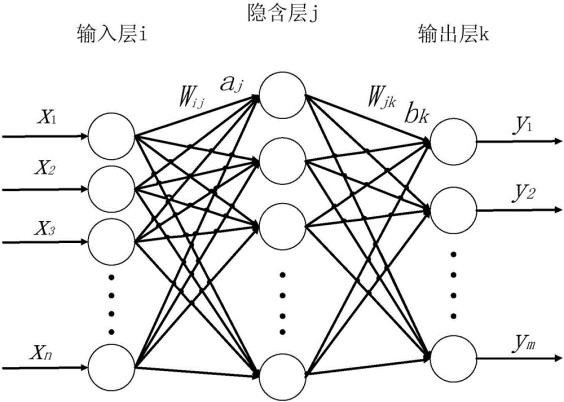
\includegraphics[scale=0.55]{三层BP神经网络结构图.jpeg}
		\caption{三层BP神经网络结构图}
	\end{figure}\par
	\textbf{(2)神经网络的建立}\par
	在一个三层 BP 神经网络中,假设输入层有$n$个神经元,输出层有$q$个神经元,隐藏层有$p$个神经元。各参数变量设置如下:\par 
	\begin{equation}
		\begin{aligned}
			\text{输入样本:}A_k=\left[ {a_1}^k,{a_2}^k,…,{a_n}^k \right] 
			\\
			\text{预期样本:}Y_k=\left[ {y_1}^k,{y_2}^k,…,{y_n}^k \right] 
		\end{aligned}
	\end{equation}
\begin{equation}
\begin{aligned}
\begin{matrix}
	\text{输入层至隐藏层的权值:}w_{ij}&		\text{隐藏层各神经元的阀值:}\theta _j\\
\end{matrix}
\\
\begin{matrix}
	\text{隐藏层各神经元的输出:}b_j&		\text{输出层各神经元的响应:}c_t\\
\end{matrix}
\\
\begin{matrix}
	\text{隐藏层至输出层的权值:}v_{jk}&		\text{输出层各神经元的阀值:}\gamma _t\\
\end{matrix}
\\
\begin{matrix}
	\text{隐藏层各神经元的输入:}s_j&		\text{输出层各神经元的输出:}l_t\\
\end{matrix}
\end{aligned}
\end{equation}\par
*注:以上各参数中,$i=1,2,…,n$ $j=1,2,…,p$ $t=1,2,…,q$  $k=1,2,…,m$\par
[1]对权值、阈值初始化,一般来说赋予$\left[ -1,+1 \right]$区间内的随机值; \par
[2]将第一组样本数据输入网络; \par
[3]通过$w_{ij}$和$\theta _j$来计算隐藏层各神经元的输入:\par
\begin{equation}
s_j=\sum{w_{ij}}\cdot a_i-\theta _j
\end{equation}\par
再通过激活函数来计算隐藏层各神经元的输出: \par
\begin{equation}
b_j=f\left( s_j \right) 
\end{equation}\par
此处使用的激活函数为sigmoid函数,即: \par
\begin{equation}
f\left( x \right) =\frac{1}{1+e^{-x}}
\end{equation}\par
[4]计算输出层各神经元的输出$l_t$: \par
\begin{equation}
	l_t=\sum{v_{jt}\cdot b_j-\gamma _t\left( j=1,2,…,p \right)}\left( t=1,2,…,q \right) 
\end{equation}\par
则输出层各神经元的响应为: \par
\begin{equation}
c_t=f\left( l_t \right) 
\end{equation}\par
[5]计算输出层各神经元的校正误差$d_t^k$: \par
\begin{equation}
d_{t}^{k}=\left( y_{t}^{k}-c_t \right) \cdot c_t\left( 1-c_t \right) \left( t=1,2,…,q \right) 
\end{equation}\par
[6]计算隐藏层的校正误差$e_j^k$:\par
\begin{equation}
e_{j}^{k}=\left[ \sum{d_{t}^{k}\cdot v_{jk}} \right] b_j\left( 1-b_j \right) \left( t=1,2,…,q \right) 
\end{equation}\par
[7]修正隐藏层与输出层之间的连接权值: \par
	\begin{equation}
	\begin{aligned}
v_{jt}\left( N+1 \right) =v_{ij}\left( N \right) +\alpha \cdot d_{j}^{k}\cdot b_{i}^{k}
\\
\gamma _t\left( N+1 \right) =\gamma _t\left( N \right) +\alpha \cdot d_{j}^{k}
		\end{aligned}
\end{equation}\par 
上式中,$N$为学习次数。\par
[8]修正输出层与隐藏层之间的连接权值: \par
	\begin{equation}
	\begin{aligned}
		w_{ij}\left( N+1 \right) =w_{ij}\left( N \right) +\beta \cdot e_{j}^{k}\cdot a_{i}^{k}
		\\
		\theta _j\left( N+1 \right) =\theta _j\left( N \right) +\beta \cdot e_{j}^{k}
	\end{aligned}
\end{equation}\par 
[9]重复[3]~[8],直至全局误差$E$小于预期误差,或学习次数大于预先定义的数值。 \par
\subsubsection{模型二的求解}
对于飞行操纵的量化处理,我们对选择的飞行数据与操纵数据进行了均值和增长率的计算,通过均值和增长率来对其进行量化。将量化的数据用MATLAB软件进行BP- 神经网络的处理,其中飞行数据为自变量$x_1,x_2,…,x_n$,操纵数据为因变量量$y_1,y_2,…,y_m$。若飞机出现超限数据$u_0$时,则可以通过该数据得到对应的操纵参数$C=\left[ y_{1a},y_{2a},y_{3a},…,y_{ma} \right] $,航空公司要求飞机的当前参数为$u\prime$,则通过求解得到对应的操纵参数为$C\prime=\left[ y_1c\prime,y_2c\prime,y_3c\prime,…,y_mc\prime \right] $,则各操纵参数的修正幅度为$\varDelta y=y_ic\prime-y_jc\prime$。\par 
	\begin{figure}[h]
	\centering
	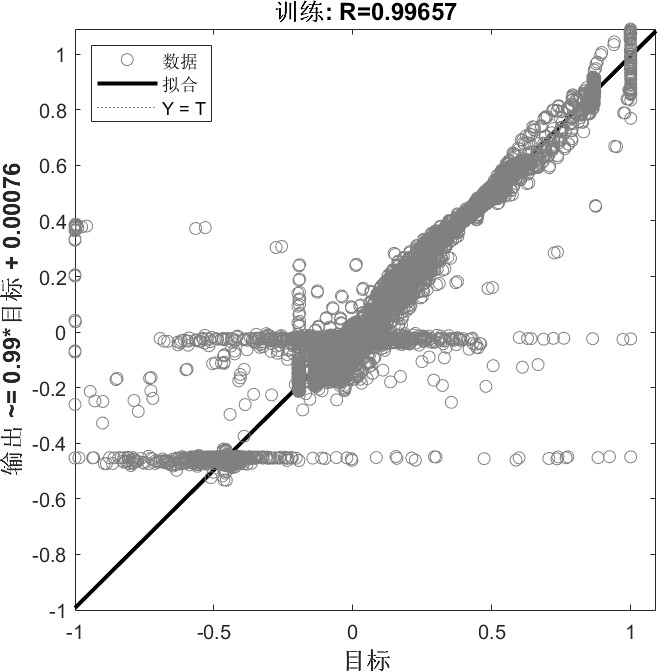
\includegraphics[scale=0.8]{BP-神经网络拟合结果.jpeg}
	\caption{BP-神经网络拟合结果}
\end{figure}\par
通过图2的拟合结果分析可知,R=0.99657 说明数据拟合结果较好。 \par
	\begin{figure}[h]
	\centering
	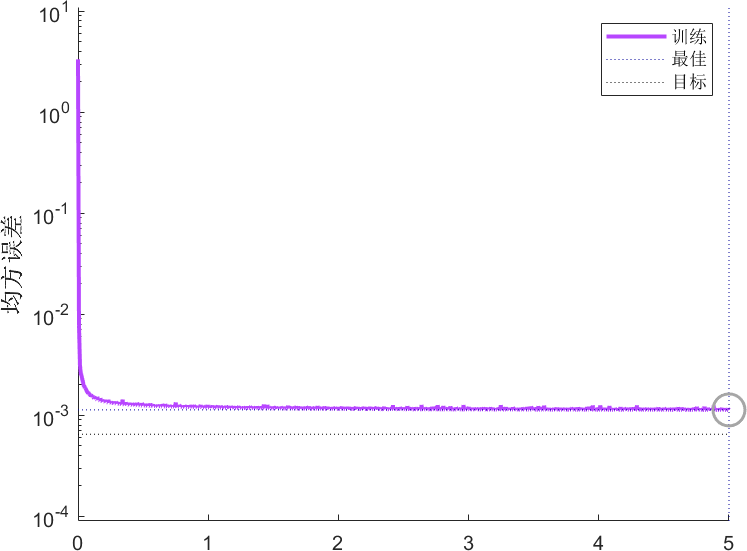
\includegraphics[scale=0.8]{均方误差.png}
	\caption{均方误差}
\end{figure}\par
由图3可知,均方误差逐渐趋于最佳值,模型处理效果较好。 \par
通过BP-神经网络训练得到飞机操纵杆数据的预测值$y_1\prime,y_2\prime,…,y_m\prime$,则存在:  \par
\begin{equation}
	W=\frac{\left| y-y\prime \right|}{y}\times 100\%
\end{equation}\par 
其中,$W$表示预测结果的相对误差。  \par
通过上述分析与计算可得使用该模型的误差较小,拟合程度较高,效果较好,该模型可用于反应飞行数据与操纵数据两者之间的关系。  \par
\subsubsection{问题三的模型建立与求解}
由于不同的超限发生的原因各不相同,因此需要得到不同超限的基本信息。结合问题分析可知,需要对附件2中不同超限进行数理分析,首先需统计各超限事件发生的概率,具体结果如表7所示。 \par
\begin{table}[!ht]
	\centering
	\caption{不同事件发生超限的概率}
	\scalebox{0.6}{
	\begin{tabular}{|l|lll|}
		\hline
		\textbf{序号} & 事件名称 & 频数 & 频率 \\ \hline
		\textbf{1} & 50 英尺至接地距离近  & 5 & 0.00011 \\ 
		\textbf{2} & 50 英尺至接地距离远  & 16692 & 0.37848 \\ 
		\textbf{3} & GPWS 警告(sink rate)  & 48 & 0.00109 \\ 
		\textbf{4} & GPWS 警告(windshear)  & 11 & 0.00025 \\ 
		\textbf{5} & High normal accel with flap (in flight) & 7 & 0.00016 \\ 
		\textbf{6} & Left of centreline below 1000ft & 1 & 0.00002 \\ 
		\textbf{7} & TCAS RA 警告  & 1 & 0.00002 \\ 
		\textbf{8} & 超襟翼限制速度 Vfe  & 3 & 0.00007 \\ 
		\textbf{9} & 低空大速度 2500ft 以下  & 30 & 0.00068 \\ 
		\textbf{10} & 低于下滑道  & 307 & 0.00696 \\ 
		\textbf{11} & 放起落架晚  & 7 & 0.00016 \\ 
		\textbf{12} & 复飞  & 5 & 0.00011 \\ 
		\textbf{13} & 高于下滑道  & 122 & 0.00277 \\ 
		\textbf{14} & 接地速度小  & 9399 & 0.21311 \\ 
		\textbf{15} & 进近坡度大 1500-500(含)ft  & 3 & 0.00007 \\ 
		\textbf{16} & 进近坡度大 200-50(含)ft  & 58 & 0.00132 \\ 
		\textbf{17} & 进近坡度大 500-200(含)ft  & 6 & 0.00014 \\ 
		\textbf{18} & 进近坡度大 50ft 以下 & 1553 & 0.03521 \\ 
		\textbf{19} & 进近速度大 50 ft 以下  & 764 & 0.01732 \\ 
		\textbf{20} & 进近速度大 500-50(含)ft  & 76 & 0.00172 \\ 
		\textbf{21} & 进近速度小 500 ft 以下  & 1 & 0.00002 \\ 
		\textbf{22} & 空中过载  & 95 & 0.00215 \\ 
		\textbf{23} & 离地速度大  & 144 & 0.00327 \\ 
		\textbf{24} & 离地速度小  & 3 & 0.00007 \\ 
		\textbf{25} & 离地仰角大  & 6 & 0.00014 \\ 
		\textbf{26} & 爬升坡度大 35-400(含)ft  & 1 & 0.00002 \\ 
		\textbf{27} & 爬升速度大 35-1000ft  & 10748 & 0.24370 \\ 
		\textbf{28} & 爬升速度小 35-1000ft  & 69 & 0.00156 \\ 
		\textbf{29} & 坡度大 400/1500ft 以上  & 12 & 0.00027 \\ 
		\textbf{30} & 起飞 EGT 超限  & 5 & 0.00011 \\ 
		\textbf{31} & 起飞滑跑方向不稳定  & 2 & 0.00005 \\ 
		\textbf{32} & 起飞坡度大 0-35(含)ft  & 131 & 0.00297 \\ 
		\textbf{33} & 起飞收起落架晚  & 1 & 0.00002 \\ 
		\textbf{34} & 收反推晚  & 155 & 0.00351 \\ 
		\textbf{35} & 抬前轮速度大  & 105 & 0.00238 \\ 
		\textbf{36} & 抬前轮速度小  & 42 & 0.00095 \\ 
		\textbf{37} & 抬头速率大  & 1 & 0.00002 \\ 
		\textbf{38} & 抬头速率小  & 19 & 0.00043 \\ 
		\textbf{39} & 未知  & 52 & 0.00118 \\ 
		\textbf{40} & 下滑道警告  & 43 & 0.00097 \\ 
		\textbf{41} & 下降率大 1000-400(含)ft  & 196 & 0.00444 \\ 
		\textbf{42} & 下降率大 2000-1000(含)ft  & 577 & 0.01308 \\ 
		\textbf{43} & 下降率大 400-50ft  & 1661 & 0.03766 \\ 
		\textbf{44} & 着陆垂直载荷大  & 281 & 0.00637 \\ 
		\textbf{45} & 着陆俯仰角大  & 17 & 0.00039 \\ 
		\textbf{46} & 着陆俯仰角小  & 401 & 0.00909 \\ 
		\textbf{47} & 着陆襟翼到位晚  & 33 & 0.00075 \\ 
		\textbf{48} & 着陆重、跳着陆  & 6 & 0.00014 \\ 
		\textbf{49} & 直线滑行速度大  & 27 & 0.00061 \\ 
		\textbf{50} & 转弯滑行速度大  & 171 & 0.00388 \\ \hline
	\end{tabular}
}
\end{table}\par
对于上表中的数据及附件2的数据可知,当事件发生概率较小时,可以认为该事件为突发事件。此时该事件不具备反映事件特征的信息值。在概率论中一般多采用0.01-0.05两个值即事件发生的概率在0.01以下或0.05以下的事件称为小概率事件。对于该题,我们取0.01作为小概率标准。则突发事件的事件名称如表8所示。 \par
\begin{table}[!ht]
	\centering
	\caption{突发事件}
	\begin{tabular}{|l|l|l|l|}
		\hline
		序号 & 事件名称 & 序号 & 事件名称 \\ \hline
		1 & 50 英尺至接地距离近 & 23 & 爬升速度小 35-1000ft \\ 
		2 & GPWS 警告(sink rate) & 24 & 坡度大 400/1500ft 以上 \\ 
		3 & GPWS 警告(windshear) & 25 & 起飞 EGT 超限 \\ 
		4 & High normal accel with flap (in flight) & 26 & 起飞滑跑方向不稳定 \\ 
		5 & Left of centreline below 1000ft & 27 & 起飞坡度大 0-35(含)ft \\ 
		6 & TCAS RA 警告 & 28 & 起飞收起落架晚 \\ 
		7 & 超襟翼限制速度 Vfe & 29 & 收反推晚 \\ 
		8 & 低空大速度 2500ft 以下 & 30 & 抬前轮速度大 \\ 
		9 & 低于下滑道 & 31 & 抬前轮速度小 \\ 
		10 & 放起落架晚 & 32 & 抬头速率大 \\ 
		11 & 复飞 & 33 & 抬头速率小 \\ 
		12 & 高于下滑道 & 34 & 未知 \\ 
		13 & 进近坡度大 1500-500(含)ft & 35 & 下滑道警告 \\ 
		14 & 进近坡度大 200-50(含)ft & 36 & 下降率大 1000-400(含)ft \\ 
		15 & 进近坡度大 500-200(含)ft & 37 & 着陆垂直载荷大 \\ 
		16 & 进近速度大 500-50(含)ft & 38 & 着陆俯仰角大 \\ 
		17 & 进近速度小 500 ft 以下 & 39 & 着陆俯仰角小 \\ 
		18 & 空中过载 & 40 & 着陆襟翼到位晚 \\ 
		19 & 离地速度大 & 41 & 着陆重、跳着陆 \\ 
		20 & 离地速度小 & 42 & 直线滑行速度大 \\ 
		21 & 离地仰角大 & 43 & 转弯滑行速度大 \\ 
		22 & 爬升坡度大 35-400(含)ft & & \\ \hline
	\end{tabular}
\end{table}\par
对于其余事件我们进行分析提取相应的特征信息值,具体事件名称如表9所示。\par
\begin{table}[!ht]
	\centering
	\caption{正常可分析事件 }
	\begin{tabular}{|l|l|}
		\hline
		\textbf{序号} & \textbf{事件名称} \\ \hline
		\textbf{1} & 50 英尺至接地距离远 \\ 
		\textbf{2} & 爬升速度大 35-1000ft \\ 
		\textbf{3} & 接地速度小 \\ 
		\textbf{4} & 下降率大 400-50ft \\ 
		\textbf{5} & 进近坡度大 50ft 以下 \\ 
		\textbf{6} & 进近速度大 50 ft 以下 \\ 
		\textbf{7} & 下降率大 2000-1000(含)ft \\ \hline
	\end{tabular}
\end{table}\par
对下表9的事件进行特征信息值的提取,如下所述: \par
50英尺至接地距离远:该事件99.8\%发生在着陆阶段;该事件发生的主要起飞机场是 68、89、16其中最主要机场是机场68占百分比为42.3\%;该事件发生的主要目的机场是68、89、27,其中最主要的是机场68占比为45.1\%;该事件在2016年发生相当于2015年偏高;发生的主要机号是26、16、23 号,其中在26号发生概率最高为3.7\%; 该事件发生的警告级别主要是2级为87.2\%。 \par
爬升速度大35-1000ft:该事件100\%发生在空中阶段;该事件发生的主要起飞机场是68、16、88,其中最主要机场是机场68占百分比为36.2\%;该事件发生的主要目的机场是68、16、89,其中最主要的是机场68占比为 51.2\%;该事件在2016年发生相当于 2015年偏高;发生的主要机号是18、71、23号,其中在 18号发生概率最高为2.7\%; 该事件发生的警告级别主要是2级为82.3\%。 \par
接地速度小:该事件100\%发生在着陆阶段;该事件发生的主要起飞机场是68、89、16其中最主要机场是机场68占百分比为40.3\%;该事件发生的主要目的机场是68、89、61,其中最主要的是机场68占比为49.5\%;该事件在2015与2016发生概率相差不大其中2015年略偏高;发生的主要机号是26、16、105 号,其中在26号发生概率最高为4.0\%;该事件发生的警告级别主要是2级为 97.9\%。 \par
下降率大400-50ft:该事件99.6\%发生在进近阶段;该事件发生的主要起飞机场是68、89、16 其中最主要机场是机场68占百分比为38.2\%;该事件发生的主要目的机场是68、89、16,其中最主要的是机场68占比为46.0\%;该事件在2016年发生相当于2015年偏高;发生的主要机号是16、23、21号,其中在16号发生概率最高为3.2\%; 该事件发生的警告级别主要是2级为 98.0\%。 \par
进近坡度大50ft以下:该事件92.2\%发生在进近阶段;该事件发生的主要起飞机场是 68、89、16其中最主要机场是机场68占百分比为34.7\%;该事件发生的主要目的机场是68、16、89,其中最主要的是机场68占比为52.6\%;该事件在2016年发生相当于2015年略偏高;发生的主要机号是105、5、20 号,其中在105号发生概率最高为3.4\%; 该事件发生的警告级别主要是2级为96.5\%。 \par
进近速度大50ft以下:该事件99.2\%发生在进近阶段;该事件发生的主要起飞机场是 68、89、16其中最主要机场是机场68占百分比为32.5\%;该事件发生的主要目的机场是68、16、27,其中最主要的是机场68占比为56.5\%;该事件在2016年发生相当于2015年偏高;发生的主要机号是69、87、74 号,其中在69号发生概率最高为3.1\%; 该事件发生的警告级别主要是2级为 92.5\%。 \par
下降率大2000-1000(含)ft:该事件 96.5\%发生在进近阶段;该事件发生的主要起飞机场是68、89、16 其中最主要机场是机场68占百分比为 52.1\%;该事件发生的主要目的机场是68、104、100,其中最主要的是机场68占比为32.0\%;该事件在2016年发生相当于2015年偏高;发生的主要机号是60、14、17号,其中在60号发生概率最高为 3.6\%;该事件发生的警告级别主要是2级为84.4\%。 \par
\subsection{问题四的模型建立与求解}
要对飞行员的技术进行科学合理的评判,可以通过该飞行员历史的飞行数据进行判断,对于其中一些重要的数据,我们可以分析出该飞行员实际操控的稳定程度,为我们衡量飞行员技术的强与弱提供了十分重要的依据,基于此并结合上述问题分析,对附件中各指标逐一分析。 \par
\subsubsection{数据预处理}
由于附件3中数据指标过多,且其中存在冗余指标,为了提高计算结果的精度,需对指标进行预处理,处理如下: \par
{1}对于固定数值的指标,不进行研究,删除处理。 \par
{2}对于表中空白的数据,不进行研究,删除处理。 \par
{3}对于表中对于所研究的目标无关的数据,不进行研究,删除处理。 \par
\subsubsection{GBDT梯度提升树}
梯度提升决策树(GBDT)是一种基于boosting集成学习思想的加法模型,训练时采用前向分布算法进行贪婪的学习,每次迭代都学习一棵CART树来拟合之前$t-1$棵树的预测结果与训练样本真实值的残差。  \par
\textbf{(1)回归树生成算法 }\par
输入:训练数据集$D$   \par
输出:回归树$f\left( x \right) $     \par
在训练数据集所在的输入空间中,递归的将每个区域划分为两个子区域并决定每个子区域上的输出值,构建二叉决策树:  \par
[1]选择最优切分变量$j$与切分点$s$,求解: \par
\begin{equation}
\min_{j,s} \left[ \min_{c_1} \sum_{x_i\in R_1\left( j,s \right)}{\left( y_i-c_1 \right) ^2}+\underset{c_2}{\min}\sum_{x_i\in R_2\left( j,s \right)}{\left( y_i-c_2 \right) ^2} \right] 
\end{equation}\par
遍历变量$j$,对固定的切分变量$j$扫描切分点$s$,选择使得上式达到最小值的对$\left( j,s \right) $;\par
[2]用选定的对$\left( j,s \right) $划分区域并决定相应的输出值: \par
	\begin{equation}
	\begin{aligned}
	R_1\left( j,s \right) =x\left| x^{\left( j \right)} \right. \leq s,R_2\left( j,s \right) =x\left| x^{\left( j \right)} \right. >s
	\\
	\hat{c}_m=\frac{1}{N}\sum_{x_i\in R_m\left( j,s \right)}{y_i},m=1,2
	\end{aligned}
\end{equation}\par
[3]继续对两个子区域调用步骤[1]和[2],直至满足停止条件;\par
[4]将输入空间划分为$M$区域$R_1,R_2,…,R_m$,生成决策树: \par
	\begin{equation}
f\left( x \right) =\sum_{m=1}^M{\hat{c}_mI\left( x\in R_m \right)}
\end{equation}\par
\textbf{(2)提升树算法 }\par
输入:训练数据集$T$ \par
输出:提升树$f_M\left( x \right) $   \par
[1]初始化$f_0\left( x \right)=0 $	   \par
[2]对$m=1,2,…,M$计算残差: \par
\begin{equation}
r_{mi}=y_i-f_{m-1}\left( x \right) ,i=1,2,…,N
\end{equation}\par
拟合残差$r_{mi}$学习一个回归树,得到$T_m\left( x \right) $,更新$f_m\left( x \right) =f_{m-2}\left( x \right) +T_m\left( x \right) $ \par                    
[3]得到回归问题提升树 \par
\begin{equation}
	f_M\left( x \right) =\sum_{m=1}^M{T_m\left( x \right)}
\end{equation}\par
\textbf{(3)GBDT算法  }\par
[1]初始化弱学习器 \par
\begin{equation}
	f_0\left( x \right) =arg\underset{c}{\min}\sum_{i=1}^N{L\left( y_i,c \right)}
\end{equation}\par
[2]对每个样本$m\i=1,2,…,M$,计算残差: \par
\begin{equation}
r_{im}=-\left[ \frac{\partial L\left( y_i,f\left( x_i \right) \right)}{\partial f\left( x_i \right)} \right] _{f\left( x \right) =f_{m-1}\left( x \right)}
\end{equation}\par
将上步得到的残差作为样本新的真实值,并将数据$\left( x_i,r_{im} \right) $,$i=1,2,…,N$作为下棵树的训练数据, 得到一颗新的回归树$f_m\left( x \right) $,其对应的叶子节点区域为$R_{jm}$,$ji=1,2,…,J$。其中$J$为回归树$t$ 的叶子节点的个数。 \par
[3]对叶子区域$ji=1,2,…,J$,计算最佳拟合值 \par
\begin{equation}
\gamma _{jm}=arg\underset{\gamma}{\min}\sum_{x_i\in R_{jm}}{L\left( y_i,f_{m-1}\left( x_i \right) +\gamma \right)}
\end{equation}\par
[4]更新强学习器: \par
\begin{equation}
f_m\left( x \right) =f_{m-1}\left( x \right) +\sum_{j=1}^J{\gamma _{jm}I\left( x_i\in R_{jm} \right)}
\end{equation}\par
[5]得到最终学习器: \par
\begin{equation}
f\left( x \right) =f_N\left( x \right) =f_0\left( x \right) +\sum_{m=1}^M{\sum_{j=1}^J{\gamma _{jm}I\left( x_i\in R_{jm} \right)}}
\end{equation}\par
\subsubsection{数据处理及结果}
基于预处理过后的数据,我们对其进行GBDT算法计算,利用SPSSPRO软件进行分析,得到的模型评估结果如表10所示。\par
\begin{table}[!ht]
	\centering
	\caption{模型评估结果}
	\begin{tabular}{|l|l|l|l|l|}
		\hline
		\textbf{} & \textbf{准确率}  & \textbf{召回率}  & \textbf{精确率}  & \textbf{F1} \\ \hline
		\textbf{训练集} & 1 & 1 & 1 & 1 \\ \hline
		\textbf{测试集} & 0.764 & 0.764 & 0.592 & 0.305 \\ \hline
	\end{tabular}
\end{table}\par
据上表可知,该数据训练集和测试集的准确率、召回率、精确率均较高,由此可知该算法对于此类数据的处理分析效果较好。\par
对于其特征重要性的簇状条形图,如图4所示。由于数据量过大本文中只呈现重
要程度位于前20的飞行参数。\par
	\begin{figure}[h]
	\centering
	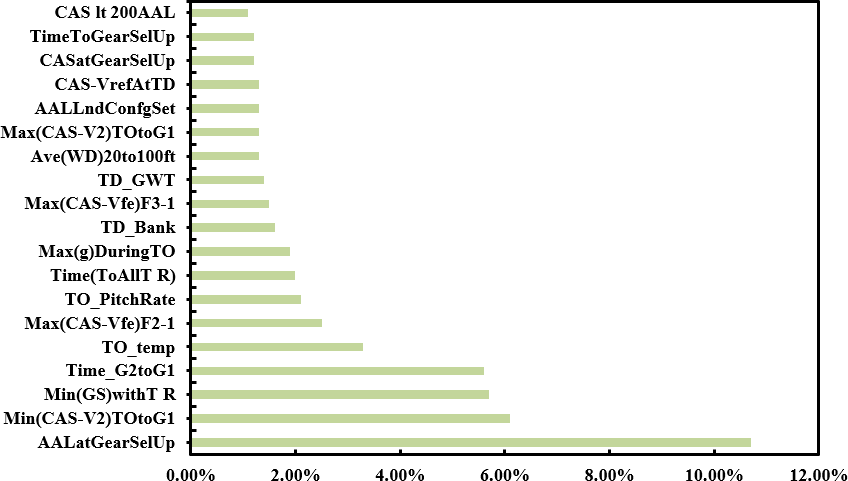
\includegraphics[scale=0.65]{重要程度前20名飞行参数.png}
	\caption{重要程度前20名飞行参数 }
\end{figure}\par
对于其最终GBDT算法最终预测结果如表11所示,由于数据量过大,在文中只展示一部分内容。\par
\begin{table}[!ht]
	\centering
	\caption{位于前 20 名的特征重要性}
	\scalebox{0.6}{
	\begin{tabular}{|lllllll|}
		\hline
		\textbf{预测结果 } & \textbf{落地主操控人员资质 } & \textbf{预测测试结果概率\_A } & \textbf{预测测试结果概率\_F } & \textbf{预测测试结果概率\_J } & \textbf{预测测试结果概率\_M } & \textbf{预测测试结果概率\_T } \\ \hline
		J & J & 0.111094909 & 0.064160320 & 0.817152673 & 0.007525633 & 0.000066500 \\ 
		J & J & 0.010298102 & 0.008205812 & 0.979858950 & 0.001626607 & 0.000010500 \\ 
		A & A & 0.999766953 & 0.000015200 & 0.000215887 & 0.000001980 & 0.000000006 \\ 
		J & J & 0.000060600 & 0.000153621 & 0.999771405 & 0.000014200 & 0.000000126 \\ 
		J & F & 0.000006100 & 0.000118154 & 0.999874149 & 0.000001590 & 0.000000013 \\ 
		J & J & 0.000003440 & 0.000650363 & 0.999343835 & 0.000002340 & 0.000000021 \\ 
		J & J & 0.116490191 & 0.345228384 & 0.501555108 & 0.036404804 & 0.000321514 \\ 
		J & J & 0.000465248 & 0.001633782 & 0.997628848 & 0.000269740 & 0.000002380 \\ 
		J & A & 0.233611682 & 0.000373771 & 0.765978248 & 0.000036000 & 0.000000318 \\ \hline
	\end{tabular}
}
\end{table} \par
通过对表11的分析可知,预测结果与落地主操控人员资质吻合程度高,由此可得该模型在基于参数的飞机技术评估方法分析飞行员技术中表现较好。 \par
\subsection{问题五的模型建立与求解}
\subsubsection{模型建立准备}
分析可用于安全预警的飞机数据,在问题二中已经对飞行数据做了处理,以问题二的指标为准,飞机操纵杆数据同上,筛选出可以用于安全预警的数据。预警模型的建立, 能利用实时飞行数据来进行处理对可能发生的安全事故做预测,可以有效减少可能发生的安全事故带来的危害,利于人们及时发现危险并解决。  \par
\subsubsection{模型建立}
若要对飞机的飞行状态进行评估,则需要以飞机标准的飞行数据为准。令飞行$t$时刻的实际飞行数据为$X_{\text{实}}$,以“实时飞行数据”技术提供的对应时刻的数据为标准数据$X_{\text{标}}$,则  \par
\begin{equation}
d_t=\left( \left| X_{\text{实}}-X_{\text{标}} \right| \right) ^2
\end{equation}\par
选择 BP-神经网络来建立预警模型,将 数据值带入 BP-神经网络模型,得到 t
时刻飞机操纵杆数据预测值$y_{\text{测}}$,则 \par
\begin{equation}
	z_t=\left( \left| y_{\text{实}}-y_{\text{测}} \right| \right) ^2
\end{equation}\par
*注:$z_t$表示$t$时刻飞机操纵杆的修正值,$y_{\text{实}}$表示$t$时刻飞机操纵杆的实际值。\par
\subsubsection{模型实施}
根据上述分析得到飞机实时数据和标准数据判断飞机偏离程度及修正值来构建实时监测,步骤如下: \par
[1]更新每个时刻的飞机实时飞行数据 \par
[2]根据实时数据与标准数据判断飞机偏离程度\par
[3]通过BP-神经网络预测操纵杆的修正值 \par
[4]下一时刻判断飞行是否结束 \par
[5]若未结束继续进入下一时刻的循环其流程图如图5所示 \par
	\begin{figure}[h]
	\centering
	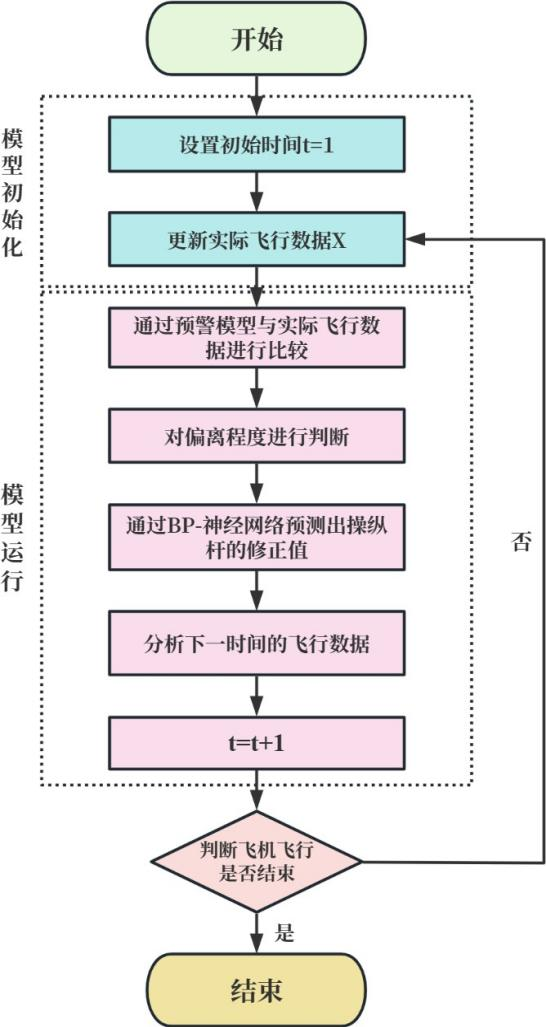
\includegraphics[scale=1]{模型流程图.jpeg}
	\caption{模型流程图}
\end{figure}\par
\subsubsection{问题的求解}
对附件1中的数据进行仿真,使用MATLAB软件在附件1的基础上进行数值修正,认为修正后的数据为飞机的标准数据,对每一时刻的飞行数据仿真如下表12所示: \par
\begin{table}[!ht]
	\centering
	\caption{飞行数据仿真}
	\begin{tabular}{|c|c|c|c|c|c|}
		\hline
		\textbf{t} & \textbf{飞行偏差}  & \multicolumn{4}{|c|}{\textbf{修正操纵值}} \\ \hline
		\textbf{1} & -0.0014 & 0.0073 & 0.0071 & 0.0073 & 0.0071 \\ \hline
		\textbf{2} & -0.001 & 0.0067 & 0.0063 & 0.0063 & -0.0065 \\ \hline
		\textbf{3} & -0.001 & -0.0056 & -0.0042 & -0.0052 & 0.0065 \\ \hline
		… & … & … & … & … & … \\ \hline
	\end{tabular}
\end{table}
\subsubsection{结果分析}
通过求解分析和仿真数据得到的结果发现此模型能够对风险识别和预警做出较为准确的判断,能够对飞行过程中的危险做出自动化的预警来预防可能的安全事故发生。 \par
\section{模型的优缺点分析}
\subsection{模型的优点}
1.	数据预处理的引入,将有助于提升数据质量,并使后续的数据处理、分析、可视化过程更加容易、有效。并且简化了处理与分析过程、提升了时效性,也使得分析挖掘的模式更容易被理解。 \par 
2.	BP-神经网络实质上实现了一个从输入到输出的映射功能,而数学理论已证明它具有实现任何复杂非线性映射的功能。这使得它特别适合于求解内部机制复杂的问题。 \par 
3.	主成分分析模型利用降维技术用少数几个综合变量来代替原始多个变量,这些综合变量集中了原始变量的大部分信息。其次它通过计算综合主成分函数得分,对客观经济现象进行了科学评价,并在应用上侧重于信息贡献影响力的综合评价。\par 
4.	GBDT算法适合低维数据它既可以处理离散值又可以处理连续值,并且该算法的调参时间短,预测的准确率相对较高,对异常值的鲁棒性较强。 \par 

\subsection{模型的缺点}
1.BP-神经网络算法的学习速度很慢,难以解决应用问题的实例规模和网络规模间的矛盾,且网络结构的选择尚无一种统一而完整的理论指导,一般只能由经验选定。\par 
2.GBDT算法对弱学习器存在依赖关系,难以对其并行计算,而且如果数据维度较高时,计算复杂度会比较高。 \par 

\section{模型的改进与推广}
\subsection{模型的改进}
对于分析结果的精度,可以再加入外部因素的影响,比如飞行的气流扰动等一些飞行过程中的外部影响,可以更加准确的反应飞机的QAR数据异常的原因。 \par 
\subsection{模型的推广}
对该建模问题建立的模型,不仅可以应用在飞机飞行安全问题的评估还可以将此模型应用到比如无人驾车安全问题的推广,对计算机操作情况进行分析预测,可以对汽车驾驶情况进行模拟比较,降低车祸事故的发生率。此外,该模型还可以对其他数据进行处理,也能够对这些数据实现有效预测,可以应用问题四建立的模型处理方式对事物的表现水平进行评级处理。该模型的处理方式对我们以后的无人智能发展具有长远意义。  \par 

%Reference
\begin{thebibliography}{40}
	\bibitem{ref1}航空安全数据[J].中国科技信息,2019(11):2-3. 
	\bibitem{ref2}[2]	叶子豪,张晓敏,刘亚飞,董朝阳.用于飞机模型参数辨识的飞行数据处理方法研究[J].航空科学技术,2022,33(08):78-87.DOI:10.19452/j.issn1007-5453.2022.08.010. 
	\bibitem{ref3}吴直龙.基于卡尔曼滤波的飞行数据处理技术研究[D].中国民用航空飞行学院,2021.DOI:10.27722/d.cnki.gzgmh.2021.000162. 
	\bibitem{ref4}何奕德,孙有朝,苏思雨,郭媛媛,杜方舟.基于MSET算法的民机QAR数据安全预警模型研究[J]. 航空计算技术,2021,51(04):86-90. 
	\bibitem{ref5}董治长,陈祖荫.教师综合水平的一种评估方法——层次分析法[J]. 中国高教研究,1985(03):80-90. 
	\bibitem{ref6}刘冰,郭海霞.MATLAB神经网络超级学习手册[M].人民邮电出版社:,201405.478. 
	\bibitem{ref7}张秀红,马迎雪,李延晖.结合主成分分析法改进后的层次分析法及应用[J].长江大学学报(自科版),2013,10(04):30-32+39.DOI:10.16772/j.cnki.1673-1409.2013.04.008. 
	\bibitem{ref8}刘冠亚.主成分-层次分析组合方法在绩效综合评价中的应用[D].云南大学,2017.
	\bibitem{ref9}桂现才.BP经网络在MATLAB上的实现与应用[J].湛江师范学院学报,2004(03):81-85. 
	\bibitem{ref10}赵雪,李晓会.面向非独立同分布数据的联邦梯度提升决策树[J/OL].计算机应用研究:1-9[2023-04-16].DOI:10.19734/j.issn.1001-3695.2022.12.0764. 
	\bibitem{ref11}张语桐.基于宏观不确定性的GBDT量化择时策略研究[D].西南科技大学,2022.DOI:10.27415/d.cnki.gxngc.2022.000065. 
	\bibitem{ref12}王国金.用于医药经济精准营销的GBDT-Logistic回归融合模型的研究[J].微型电脑应用,2022,38(10):171-174. 
	\bibitem{ref13}刘向前,安端阳,张卓昆,岳承恩,王梦迪.激光诱导击穿光谱结合RFE-GBDT算法定量分析稀土矿石中的Fe和Y[J],2023,52(03):20-25.DOI:10.16283/j.cnki.hgkwyjg.2023.03.004. 
	\bibitem{ref14}孙一兵.浅议BP网络的优缺点及改进[J].科技创新导报,2009,(24):18 
	\bibitem{ref15}王心逸.基于GBDT算法的大数据风控模型研究[J].郑州航空工业管理学院学报,2020,38(05):108-112. 
	
\end{thebibliography}
\newpage
\newgeometry{left=1.50cm,right=0.5cm,top=3.00cm,bottom=3.0cm}	%修改附录代码的几何页面

\begin{center}
	\sihao \heiti 附录1
	\fontsize{10pt}{16pt}		\selectfont	
	\begin{lstlisting}[ language=MATLAB,numbers=left,numberstyle=\tiny,keywordstyle=\color{blue!70},commentstyle=\color{red!50!green!50!blue!50},frame=shadowbox, rulesepcolor=\color{red!20!green!20!blue!20},escapeinside=``,xleftmargin=2em,xrightmargin=2em,aboveskip=1em] 
		'BP-神经网络' 'MATLAB环境'	
	\end{lstlisting}
	\begin{lstlisting}[ language=MATLAB,numbers=left,numberstyle=\tiny,keywordstyle=\color{blue!70},commentstyle=\color{red!50!green!50!blue!50},frame=shadowbox, rulesepcolor=\color{red!20!green!20!blue!20},escapeinside=``,xleftmargin=2em,xrightmargin=2em,aboveskip=1em] 
		clc clear
		A=[-0.00122	-0.00144	……	34.0576];
		y=[0 1.00117000000000	-0.351600000000000 …… 3.316666667]'%%%因变量的数据
		
		[n1,n]=size(A) %%%%自变量的个数
		[m,m1]=size(y) %%%%因变量的个数
		p=A'; %将所有自变量合并得到输入数据矩阵
		t=y; %将所有因变量合并目标数据矩阵
		%利用 premnmx 函数对数据进行归一化
		
		[pn,minp,maxp,tn,mint,maxt]=premnmx(p,t); % 对于输入矩阵 p和输出矩阵 t 进行归一化处理
		u=ones(n,1);
		dx=[-1*u,1*u];	%归一化处理后最小值为-1,最大值为 1
		%BP网络训练
		net=newff(dx,[n,7,m],{'tansig','tansig','purelin'},'tra ingdx'); %建立模型,并用梯度下降法训练.
		net.trainParam.show=1000;	%1000 轮回显示一次结果
		net.trainParam.Lr=0.05;	%学习速度为 0.05
		net.trainParam.epochs=50000;	%最大训练轮回为 50000次
		net.trainParam.goal=0.65*10^(-3); %均方误差
		net=train(net,pn,tn); %开始训练,其中 pn,tn分别为输入输出样本
		
		%利用原始数据对 BP 网络仿真
		an=sim(net,pn);	%用训练好的模型进行仿真a=postmnmx(an,mint,maxt); % 把仿真得到的数据还原为原始的数量级;
		pnew=[p]; %%输入自变量的参数,每一行表示一个自变量,列数表示预测的个数
		pnewn=tramnmx(pnew,minp,maxp); %利用原始输入数据的归一化参数对新数据进行归一化;
		anewn=sim(net,pnewn); %利用归一化后的数据进行仿真;
		anew=postmnmx(anewn,mint,maxt) %把仿真得到的数据还原为原始的数量级;
		
		wucha=abs(t-anew)./t %%%相对误差
		
	\end{lstlisting}
\end{center}
\newpage
\begin{center}
	\sihao \heiti 附录2
	\fontsize{10pt}{16pt}		\selectfont	
	\begin{lstlisting}[ language=MATLAB,numbers=left,numberstyle=\tiny,keywordstyle=\color{blue!70},commentstyle=\color{red!50!green!50!blue!50},frame=shadowbox, rulesepcolor=\color{red!20!green!20!blue!20},escapeinside=``,xleftmargin=2em,xrightmargin=2em,aboveskip=1em] 
		'基于BP-神经网络的仿真模拟' 'MATLAB环境'	
	\end{lstlisting}		
	\begin{lstlisting}[ language=MATLAB,numbers=left,numberstyle=\tiny,keywordstyle=\color{blue!70},commentstyle=\color{red!50!green!50!blue!50},frame=shadowbox, rulesepcolor=\color{red!20!green!20!blue!20},escapeinside=``,xleftmargin=2em,xrightmargin=2em,aboveskip=1em] 
		clc clear
		A=[ -0.00122	-0.00144	……	34.0576];
		
		y=[ 0 1.00117000000000	-0.351600000000000 …… 3.316666667]'%%%因变量的数据
		
		[n1,n]=size(A) %%%%自变量的个数[m,m1]=size(y) %%%%因变量的个数p=A'; %将所有自变量合并得到输入数据矩阵t=y; %将所有因变量合并目标数据矩阵
		%利用 premnmx 函数对数据进行归一化
		
		[pn,minp,maxp,tn,mint,maxt]=premnmx(p,t); % 对于输入矩阵 p和输出矩阵 t 进行归一化处理
		u=ones(n,1);
		dx=[-1*u,1*u];	%归一化处理后最小值为-1,最大值为 1
		%BP网络训练net=newff(dx,[n,7,m],{'tansig','tansig','purelin'},'tra ingdx'); %建立模型,并用梯度下降法训练.
		
		net.trainParam.show=1000;	%1000 轮回显示一次结果
		net.trainParam.Lr=0.05;	%学习速度为 0.05
		net.trainParam.epochs=50000;	%最大训练轮回为 50000次
		net.trainParam.goal=0.65*10^(-3); %均方误差
		net=train(net,pn,tn); %开始训练,其中 pn,tn分别为输入输出样本
		
		%利用原始数据对 BP 网络仿真
		
		an=sim(net,pn);	%用训练好的模型进行仿真a=postmnmx(an,mint,maxt); % 把仿真得到的数据还原为原始的数量
		级;
		pnew=[0.62 0.42
		0.74
		0.33
		1.05
		]; %%输入自变量的参数,每一行表示一个自变量,列数表示预测的个数
		pnewn=tramnmx(pnew,minp,maxp); %利用原始输入数据的归一化参数对新数据进行归一化;
		anewn=sim(net,pnewn); %利用归一化后的数据进行仿真;
		anew=postmnmx(anewn,mint,maxt) %把仿真得到的数据还原为原始的数量级;
	\end{lstlisting}
\end{center}
\end{document}